\chapter{Methodology}


\section{Requirements}
% This should state, in a more detailed way, the objectives of the project by requirement and the analysis should break the problem down into manageable steps. There may be more than one suitable approach; the analysis may cover more of the area than is finally implemented. Testing and evaluation should be given due consideration. It is important that you state how you will evaluate your work. For a design project it is appropriate to consider testing at the same time as specification.

The main requirement of this dissertation is the comparison between the Dynamic Similarity hypothesis and a simulated model, in order to establish whether a simulated gait still conforms to the values seen in the Dynamic Similarity hypothesis. For this to succeed, a valid robotic environment is required, this could take the form of a real quadruped robot or a physics simulation of a quadruped robot. If a physics environment is used, the robotic model must be based on a real life counterpart to allow for direct comparisons between real examples, as it may skew the results of the investigation to use a unrealistic model. 

This will indicate that the mathematical methods of generating gaits used in this dissertation would be valid for a real robot and that robots follow the rules of Dynamic Similarity outlined in \cite{Alexander1983}.

Although evaluating a range of different gaits is optional, it would be useful to investigate whether the same difference between cursorial walking and faster gaits is seen, as this would further prove the results. This could be done through the results found in \ref{table:froude}, through investigating Stride Length.

% useful to see whether the same issues occur as found in \cite{Rutishauser2008}, wherein faster gaits broke down more easily and produced slower movement than a walking gait.
 

\section{Analysis}
In order to break down the problem into easily manageable steps, The analysis stage has been separated into the creation of a Central Pattern Generator, the implementation of the Central Pattern Generator in a robotic environment. Additionally, a large portion of the analysis will include an analysis on the  evaluation of the gait against the Dynamic Similarity Hypothesis.

\subsection{Central Pattern Generator}
Initially, this dissertation wishes to focus on the CPG design, due to it being an integral part of the project. Additionally, many many of the methods found create the CPG first, followed by the implementation of the CPG in a robotic environment. 

There is the possibility of designing the motor actions separately, and use an evolutionary technique similar to the muscular skeletal model found in \cite{}. This has shown to work extremely well on a muscular skeletal model, and produces realistic walking movements for bipeds. However this sort of technique would be limited to off-line training, making it unsuitable for conversion to a real robot, which will have to deal with real-time processing constraints. A mixture of training with real-time feedback could be applicable, similar to the method seen in \cite{Zhang2018}, which uses a mixture of processing based on visual data along with details about current footfall, but this may be outside of the scope for this dissertation. This design is additionally based on agent control, which is not necessary for comparison.

A method which may be more appropriate for gait generation would be through the use of non-linear coupled oscillators. These seem to be widely used in both gait generation and the control of other Central Pattern Generators. This would provide this method with additional potential applications. There are many potential ways of creating a coupled central pattern generator, from the use of a Stein neuronal model, a Fitzhugh-Nagmo or a Van der Pol oscillator. Both the Stein neuronal and the Fitzhugh-Nagmo models are based on replicating neuronal movement. However, far more of the research found has used the Van der Pol oscillator in replicating natural systems, and as such, the implementation of a Van der Pol Oscillator seems to be most appropriate for this model.

Multiple different examples of Van der Pol coupling have been found that generate successful quadruped gaits. In order to investigate which are most suitable for the model, a round of testing will be performed by replicating the matrix values found. Successful gaits could be tested by calculating the phase difference between oscillators. As different gaits can be categorized by the phase differences between limbs a successful coupled gait would produce the same phase differences as that seen in mammals, an example of these differences can be seen in . As the time period of a van der pol oscillator is the same as that of sin, this can be examined by comparing the phase differences to different gait generations seen in ()). This will allow us to evaluate whether the coupling links produce correct gaits.

A potential issue that may occur when recreating the gaits is balancing, as there are a huge amount of potential balancing issues that can exists with a quadruped robot, and the work needed to fix these issues \citep{Meng2015}, would be outside the scope of the dissertation. However, as the open cat already deals with balancing issues outside of the gait methodology, it would provide a solution to these issues.


\subsection{Robotic Environment}
In order to compare results with Dynamic Similarity, an environment is required for the implementation and testing of a quadruped gaits. This in turn requires either a real robot or a simulated robot based on a real counterpart. This is in  order to reduce the effects that possibly inaccurate models may have on the final results. Using a real robot has the benefit of allowing us to perform the same measurements as seen in Dynamic Similarity. One of the initial main issues was how to find a quadruped robot that is both within the scope of the dissertation (as due to the complexity of a quadruped, it is not within the scope of this dissertation to be able to build one from scratch), and which is open source enough to allow for gait re-wiring. One of the suitable candidate for this is \cite{Li2018}, through contact with the creator, information was gathered on how to edit and add new gaits for the robot. However, this would add an extra complexity to the dissertation,  may produce some issues with measurement accuracy.  This can be seen in \cite{Collins2018}, as when using "Multi-Joint Movement" of a gripper robot it will "follow the motion capture path closely with an accumulated  error of $\pm{5.5-6}$   metres  Although this may be a small error for a motion gripper robot, when facing periodic and time necessary procedures such as gait reproduction small errors in measurements may compound and produce inaccurate movements which in turn may effect the comparison of the system between a real mammal.

The implementation of a real robot could additionally pose issues with real-time processing which could adversely effect results. This would be the main benefit of using a simulation, as it would allow an investigation of gaits without the constraints of real-time simulation. A physics engine such as PyBullet allows the running of a simulation in step simulation mode so as to reduce the effects of processing time. Furthermore, this allows for more efficient and faster data analysis, as automatic data graphing can be easily made, with larger data-sets gathered for evaluation. A robot may need to have manual data-collection for each experiment ran, and the equipment necessary to make a scientific evaluation may not be readily available. However, the implementation of a simulation instead of a real robot also means that the data may not apply directly to real life,  as model information may not be perfect, and the simulation may struggle with perfectly representing friction or forces.  


\subsection{Evaluation of Work}



\cite{Carr2016} provides information on how to evaluate between normal and abnormal dog gaits. This lets us know that purely visual observation of gaits cannot be enough to recognize whether a gait is normal or abnormal, as when attempting to identify abnormal gaits by eye, an observer ``\textit{only identified 11\% of the 131 dogs that were 6 months post surgery}''. However, \cite{Carr2016} contains some limitations, with part of the analysis includes subjective gate analysis. Since this method is used for finding medical issues with dogs, it may be specific to dog gaits.

\citep{Righetti2015} uses multiple evaluation methods in order to find Kinematic and gait similarities between infants and quadrupeds. There are a large amount of limitations with this study due to the very small amount of subjects tested. However, this does provide a potential method of evaluation, through the use of a Spearmann Correlation. This correlation can be seen to find how our different parameters cluster.

The main hypothesis that will be tested against is whether the Froude numbers found for gaits in nature are similar to those seen in generated oscillator movement. In order to do this, The robot must be evaluated over combinations of parameters that generate successful gaits, who's Froude numbers will be compared against those found in Dynamic Similarity.


\cite{Rutishauser2008} shows a potential method of gathering these parameters, through the use of a systemic search. By evaluating against a range of swing angle time periods parameters and stance time periods angles, a valid range of angles is found. Although this is not a way of evaluating how successful a gait is, it could provide a useful guideline in order to work out our ranges of testing parameters.

% In order to showcase similarity between cursorial gaits \cite{Alexander1983} defined two separate subsets: walking, which occurs at Froude numbers below 0.4 and faster gaits, which occur above 0.4. Animals performing gaits have been described the equation \ref{froude:equation}, with x representing values of relative stride lengths. \cite{Carr2016} defines Stride Length as the distance from one step to the next step of the same leg.  

 By calculating the percentage of values that lie within the ranges seen in \cite{Alexander1983}, an initial result can be seen as to whether the Dynamic Similarity hypothesis holds for the majority of values found. This could be done by comparing against maximum Froude numbers. 

By taking a normal distribution of the results, an investigation can be made as to whether the results lie within the same ranges given a certain variation.This will show that a simulated oscillator shows similar results to those seen in nature. 

A more detailed analysis can be done through equation \ref{froude:equation} with values from table \ref{table:froude}. By calculating the Stride Length and Froude number of our calculated gaits, it could be evaluated to the results found in Dynamic Similarity through the use of a paired t test. 



% The results will be evaluated through multiple methods. We wish to intially examine the differences between different gaits, and whether certain gaits such as trotting or bounding are more effective and produce faster gaits than walking at certain speeds, rotations or forces used.


% \subsection{Robot and Simulation}

% Due to this, we are choosing to focus on running a simulation of the machine learning methods outlined above first, as we still believe it will hold scientific merit, if done correctly. This is due to the large precision required to monitor gaits, this can be done easily through the simulation, but would require a large setup for a real life robot application.

% We will still attempt to procure a robot that would be valid for use and experimentation, however, that will be a secondary focus, instead of a main goal.
\section{Design}

For the implementation of a CPG, the use of a coupled non-conservative oscillator was decided on, due to it's successful implementation in gait generation and relative simplicity. Although there are multiple potential methods of generating these, a Van der Pol oscillator was decided on, due to it being a common method seen in reconstruction of natural systems. 

This produces a non-linear oscillation, and could be used successfully to model gaits. However this design of a Van der Pol oscillator contains limited control, with the only parameters being $\alpha$, as seen from equation \ref{froude:equation}. 
% This should explain the design technique chosen (and justify why it is appropriate) from the various ones available; it should select a suitable subset of the things described in the analysis chapter and develop a design. Where trade-offs exist between different designs, the chosen approach should be justified. Suitable diagram-techniques (e.g. UML, other drawings) should be used where appropriate. If a method is applied selectively, explain which parts were used and why. Experimental projects should pay careful attention to control conditions, samples selected, etc. to ensure a valid result.


% \subsection{Van der Pol Oscillators}
% \subsection{}


 PyBullet was decided as the physics engine for this dissertation, due to it's high accuracy when converting to real life robotics \cite{Collins2018s} compared to other physics simulations, as well as it containing previous working examples of replication of quadruped gaits. This can be seen through the implementation of the Minotaur walking using deep learning methods seen in \cite{Tan2018},  as well as the recent implementation of the Stoch quadruped by \cite{Singla2018}. This makes it a suitable choice for the implementation of a quadruped robot.


% In order to compare against the equations seen in \cite{Alexander1983}.

% Relative Stride Length will be calculated as the distance an animal walks in a single stride. This will be derived from the angle of rotation of the robot, as the relative stride length can be estimated through \ref{eq:relative} seen below. This will provide an estimate for relative stride length over time, and will allow direct compare against the results seen in Alexander's research. 


% This will use Froude number information from \cite{Alexander1983} to test at a variety of different gaits, e.g using  Froude Numbers below 0.4 for walking, as well as 1.0 on wards for faster gaits, as these have been shown in \cite{Alexander1983} to generate walks and faster gaits (trots, gallops) respectively.

% This will be compared with the footfall seen in table 1 of \cite{Robilliard2007}, and compared to the basic footfall information, for example, footfall contact order, number of limbs in contact with the ground, as well as presence of an aerial phase.

% This will serve as a basic check for gait success, before moving on to more robust and objective experimentation.

% The second test will involve replicating the graphs seen in \cite{Alexander1983}. We will test against the equations seen in table II, more specifically, the relative stride length for Cursorial mammals, the fore duty factor and the hind duty factor. 

% We will attempt to replicate the experiments seen in \cite{Alexander1983}, and evaluate the results against the equations found. This will be done by evaluating against the Standard Deviation factor found. For additional, and more specific gait information, the values seen in \cite{Fischer2002} will be used to evaluate against, due to the large amount of specific data contained, it will allow for testing the simulation against specific measurements.

% The final experiment performed will be similar in scope to the previous, but focusing instead on gait transitions. As seen in \cite{Alexander1983}, there is a large amount of data available on where a gait transition from a walk to a trot should occur, and comparing that to data found in \cite{Maes2013}, we can therefore extrapolate whether our simulated animal is performing gait transition in a correct way.

% This is the final experiment, as it relies on the passing of the previous two. It will be evaluated in the same methods shown in \cite{Maes2008}. For an objective comparison value, the equations found in \cite{Alexander1983} for gait transition will be used.

\section{Implementation}
\subsection{Central Pattern Generator}



Initially, in order to investigate the dynamics of the Van der Pol oscillator,  the equation seen in \ref{vanderpol:pure} was implemented. This resulted with the dynamics seen in \ref{fig:vandynamics}. 


\begin{figure}
    \centering
    \includegraphics[width=0.7\textwidth]{USFD_Academic-_Report_LaTeX-Template/figures/oscillatoroutput.png}
    \caption{Dynamics of Van der Pol oscillator}
    \label{fig:vandynamics}
\end{figure}


The modified implementation of the Van der Pol oscillator was derived from \cite{}. Coupling weights have been implemented as a scalar value, with inhibitory coupling represented by negative values, and The potential methods of coupling can be seen through \ref{}, with the corresponding matrix shown in \ref{mat:coupling}

\begin{figure}
    \centering
    $\begin{bmatrix}
    0 & fr \rightarrow br & fr\rightarrow fl & fr\rightarrow bl \\
    br\rightarrow fr & 0 & br\rightarrow fl & br\rightarrow bl \\
    fl\rightarrow fr & fl\rightarrow br & 0 & fl\rightarrow  bl \\
    bl\rightarrow fr & bl\rightarrow br & bl\rightarrow fl & 0 
    \end{bmatrix}$
    \caption{Matrix showcasing coupling of limbs (fr refers to Front Right limb, bl refers to Back Right, etc)}
    \label{mat:coupling}
\end{figure}


Although the coupling methods seen in \cite{} and \cite{} use mainly the same methods of coupling for gaits such as trotting and bounding, they use two different matrices for walking gaits. However we found that the implementation found in \cite{} did not produce gaits with the phase relations found in \cite{}. In order to measure the results of different gaits, walking, trotting and bounding will be investigated, this is due to them each having separate. This is in order to get a variation of values . These can be represented respectively by figures.

\begin{figure}
\[
\begin{bmatrix}
0   & -l & l  & -l\\
-l   & 0 & -l  & l\\
-l   & l & 0  & -l\\
l   & -l & -l  & 0\\
\end{bmatrix}
\begin{bmatrix}
0   &  -l & -l  & l\\
-l   & 0 & l  &  -l\\
-l   & l & 0  & -l\\
l   & -l & -l  & 0\\
\end{bmatrix}
\begin{bmatrix}
0   & l & -l  & -l\\
l  & 0 & -l & -l\\
-l   & -l & 0  & l\\
-l  & -l & l  & 0\\
\end{bmatrix}
\]
\caption{Coupling weights from left to right: Walking, Trotting, Bounding.}
\end{figure}

The final equation  of the modified Van der Pol oscillator with coupling can be seen in equation \ref{}, with the related python code snippet found in \cite{}. 

\begin{equation}
\ddot{x} + \alpha(x^2 - 1)\dot{x} + x = 0
\label{vanderpol:pure}
\end{equation}

\begin{figure}

\begin{lstlisting}[frame=single]
import numpy as np
from scipy.integrate import odeint
mu = 1, p = 2, w = 20, l = 1
t_s = 0.01, count = 0
s_y = [1,1,1,1],s_x = [0,0,0,0]
n_y = [0,0,0,0],n_x = [0,0,0,0]
lamb = [ [0, -l, l, -l],
          [-l, 0, -l, l],
          [-l, l, 0, -l],
          [l, -l, -l, 0]]
def vdp(x, t):
    x0 = x[1]
    x_ai =x[0]
    for j in range(4):
        x_ai += x[0]-(lamb[current_i][j]*start_x[j])
    x1 =  mu * ((p - (x_ai** 2.0))* x0) - x_ai*w
    return np.array([x0, x1])
    
while (c <= 10):
    c += t_s
    for i in range(4):
        current_i = i
        osc= odeint(vdp, [s_y[i], s_x[i]], [c-t_s, c])
        x = osc[1][1]
        y = osc[1][0]
        n_y[i] = y
        n_x[i] = x
    s_y = new_y
    s_x = new_x
\end{lstlisting}
\caption{Python implementation of coupled Central Pattern Generator }

\end{figure}
% \begin{figure}
% \begin{subfigure}{.5\textwidth}
%   \centering
%   \includegraphics[width=.8\linewidth]{image1}
%   \caption{1a}
%   \label{fig:sfig1}
% \end{subfigure}%
% \begin{subfigure}{.5\textwidth}
%   \centering
%   \includegraphics[width=.8\linewidth]{image2}
%   \caption{1b}
%   \label{fig:sfig2}
% \end{subfigure}
% \caption{plots of....}
% \label{fig:fig}
% \end{figure}

% \begin{figre}
%     \begin{subfigure}
%         \centering
%         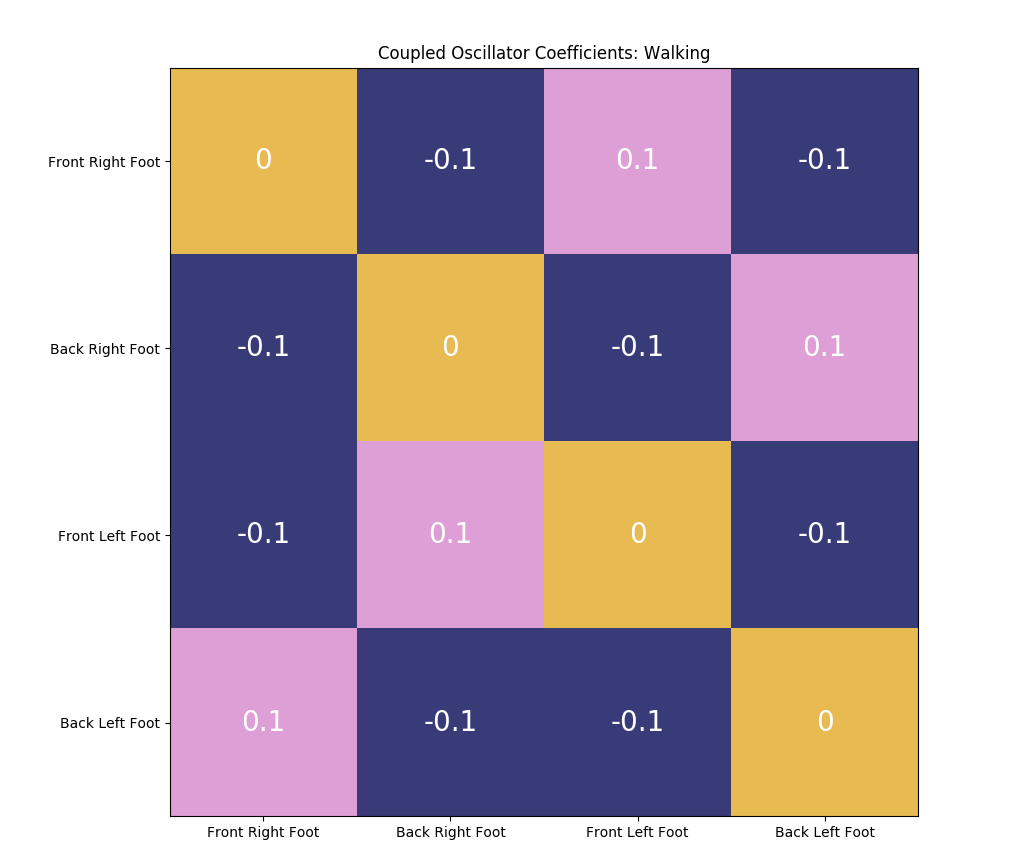
\includegraphics[width=0.33\textwidth]{USFD_Academic-_Report_LaTeX-Template/figures/walkingmatrix.png}
%         \caption{Walking Coupling Coefficients Matrix}
%         \label{fig:walk}
%     \end{subfigure}
    
%     \begin{subfigure}
%         \centering
%         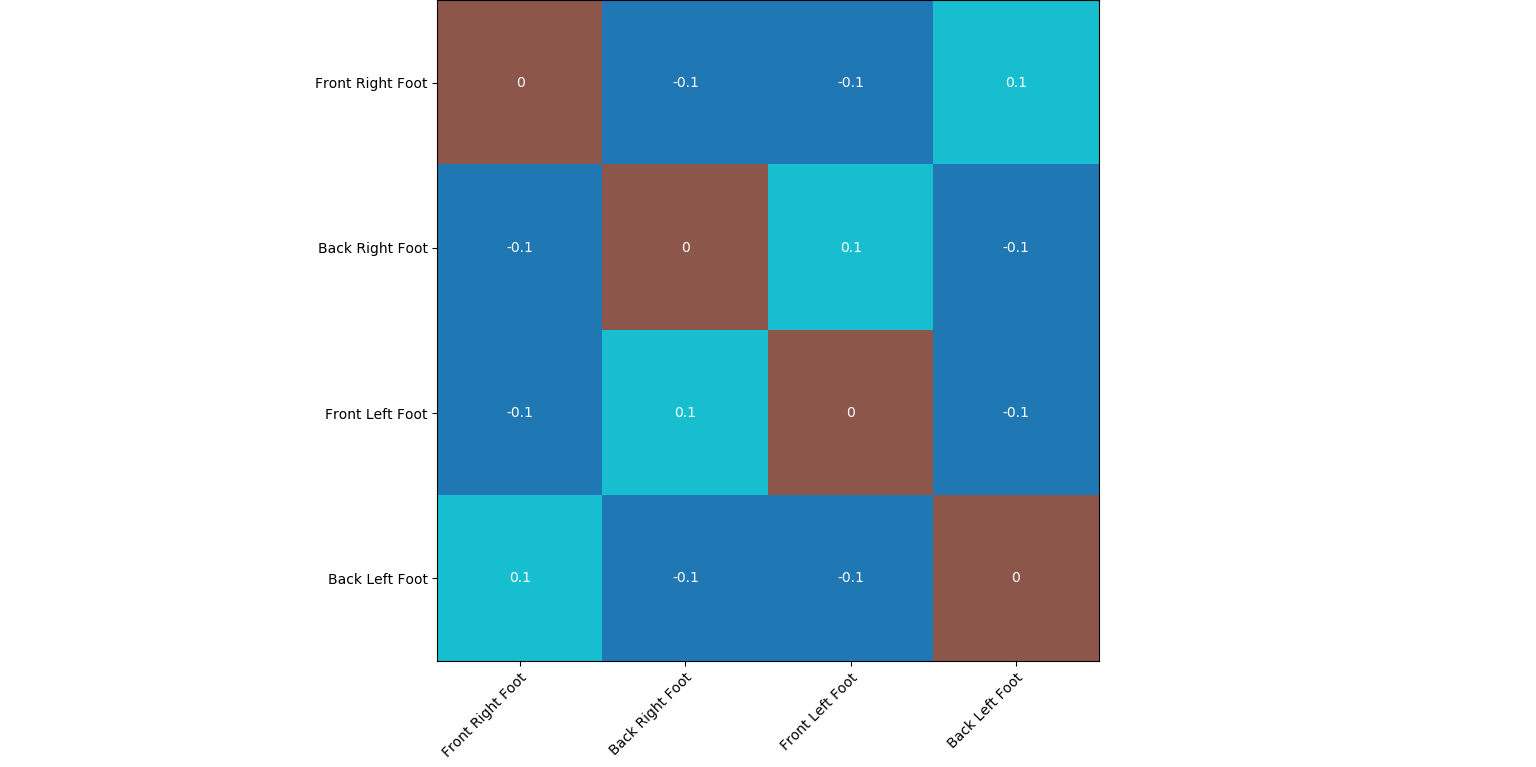
\includegraphics[width=0.33\textwidth]{USFD_Academic-_Report_LaTeX-Template/figures/trotosc.png}
%         \caption{Walking Coupling Coefficients Matrix}
%         \label{fig:walk}
%     \end{subfigure}
    
    % \begin{subfigure}
    %     \centering
    %     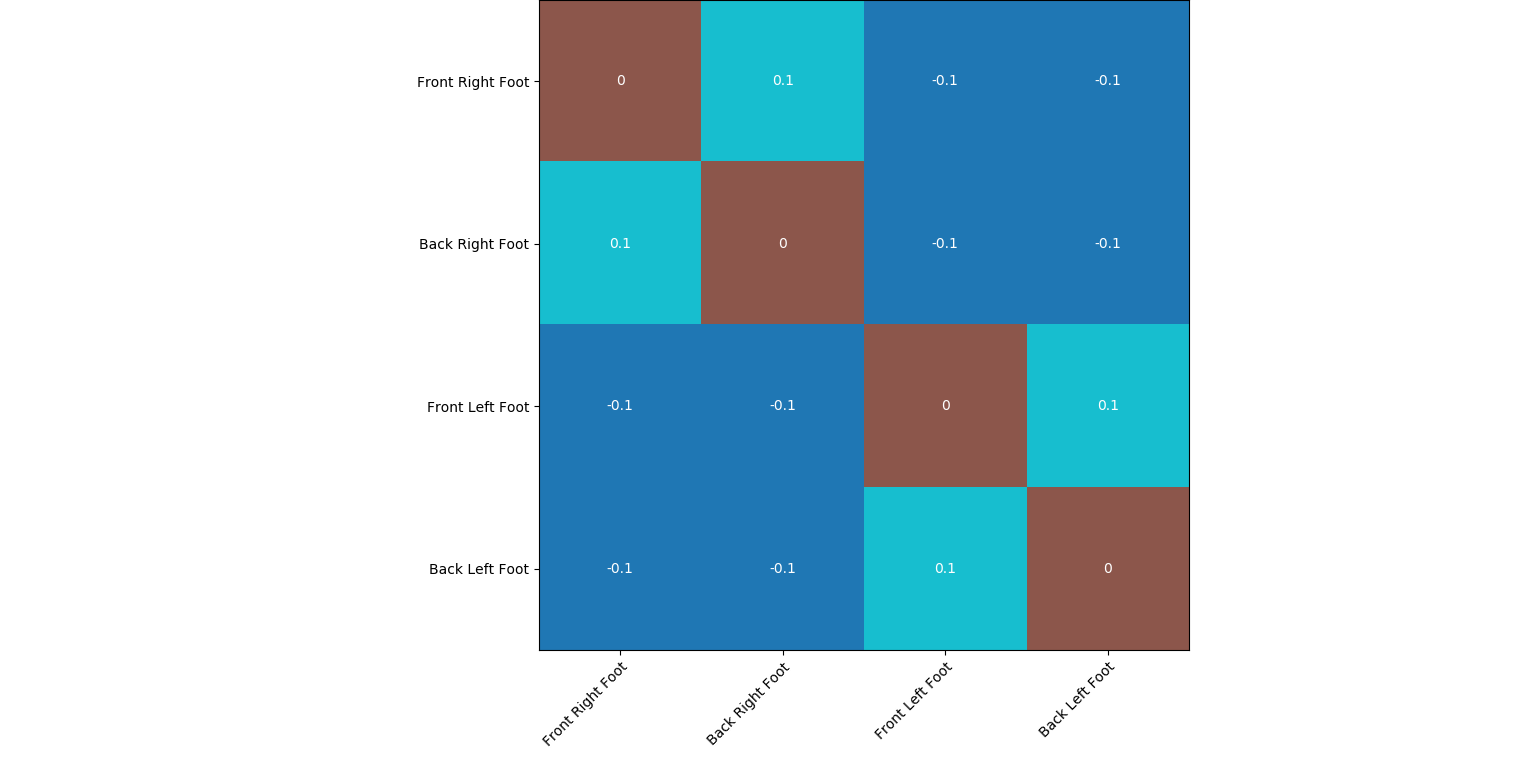
\includegraphics[width=0.33\textwidth]{USFD_Academic-_Report_LaTeX-Template/figures/osc_bound.png}
    %     \caption{Walking Coupling Coefficients Matrix}
    %     \label{fig:walk}
    % \end{subfigure}
% \end{figure}

After the implementation of the coupled Van der Pol generator to represent a CPG, the next stage of implementation is creating a robotic environment to investigate gaits.

\subsection{Robotic Environment}
This paper uses PyBullet for the creation of robotic simulation. PyBullet is a free open source physics engine which has shown success in simulating gait movement in this past. Recently, PyBullet was used in order to implement learned quadruped locomotion in \cite{Singla2018}. Additionally, investigation by \cite{Collins2018} has shown PyBullet to have extremely accurate conversion from a simulation to an actual robot, making the simulation the most appropriate for evaluating against real life values.

The robot used in this experimentation will be the Laikago robot, due it containing limbs in the Para-Saggital plane, making it a model of a Cursorial mammal. In addition using Deep Mimic, this has shown to recreate gaits successfully. 

The most appropriate form of simulation found is PyBullet's step simulation mode. PyBullet contains both step-simulation and real-time simulation. Real-time simulation replicates the processing over the current processor, while step simulation runs the next frame of simulation each time it is called. Step simulation was found to be the most appropriate as it will reduce the effects of computer processing in real time simulation on the robot. When investigated over using PyBullet's real-time option, the addition of extra monitoring changed the simulation time. This could cause issues with results testing as over time, the simulation may change due to extra processing strain on PyBullet.


% Each experiment has been repeated 10 times, and ran for 10000 iterations at time-steps of 1/500. 

Initially, before parameter testing, a successful gait was generated using the above Central Pattern Generator through values found in previous research, and trial and error. This was done in order to evaluate potential issues with the CPG design before experimentation. 

One of the issues seen with gait generation was rotation of the robot over time. This can be seen in \ref{fig:rotation}. This may be due to the lack of real time feedback of the robot, stopping the Laikago robot from correcting itself. An issue was found with the Laikago model, wherein the robot's centre of gravity was leaning to the side due to a mistake with motor masses. This issue was fixed, and the creator of PyBullet was contacted with the fixed version. Although this reduced rotation over time, it did not remedy the issue fully. As this would not be appropriate for a testing circumstance, due to the effects tilting may have on correctly finding distance travelled over time.

In order to investigate the difference between imaginary and actual oscillator values, the imaginary oscillator was transposed into the real oscillator, based on an inverse transposition at the end of 10000 iterations. An example of this transposition can be seen in \ref{}.  

\begin{figure}
    \centering
    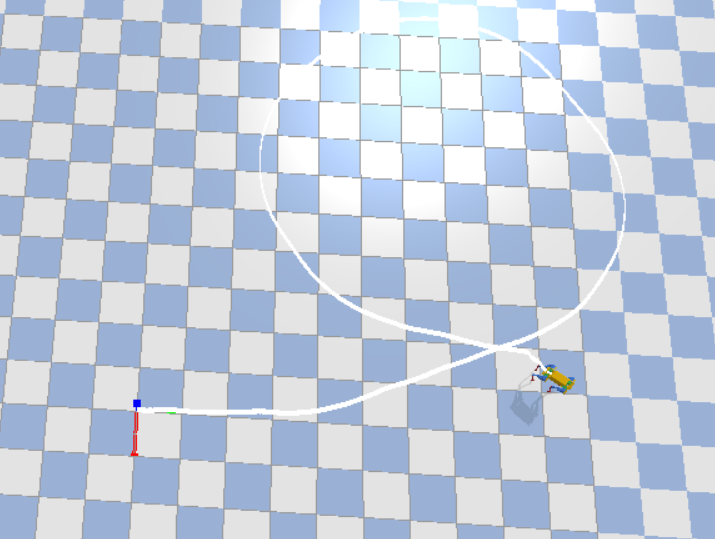
\includegraphics[width=0.65\textwidth]{USFD_Academic-_Report_LaTeX-Template/figures/rotation_over_time.png}
    \caption{Change in rotation over time. Path of robot indicated by white line}
    \label{fig:rotation}
\end{figure}

\section{Testing}
with a T test being ran between the two values, table \ref{} was found. The difference between the two values where found to be mostly negligible, and can be seen in \ref{fig:ttests}. Due to the extremely small P-values found in the T-tests, it shows that there is not a large effect on virtual oscillator values being moved into simulated limbs. This change may be far larger for implementation into an actual robot, and as such, may cause issues with gait generation, however, the extremely low p-values found suggests that there is potential in accurate conversion for actual robots. 

In order to create a suitable testing environment, two walls where created on either sides of the robot in order to reduce measurement complexity and reduce the effect of balancing issues may have on the robot, as issues with the robot collapsing in the middle of its gait may cause inaccurate measurements of Froude number. This reduces the effects seen by the robot tilting over time.

A similar method of parameter search as found in \cite{Rutishauser2008} was decided due to needing a wide range of different Froude number values when comparing against the Dynamic Similarity Hypothesis. This was through the use of evaluating against a large combination of parameters and building a matrix table of successful results. Initially, we investigated two main parameters, max-force and speed of oscillations against a full set of gaits. 

As can be seen from \ref{}, this found that the minimum force value for all gaits 15N. Below this, the robot could not sustain it's own weight. Above 120N all gaits, however, both trotting and walking experienced cut offs at both 80N.

A slight change has been  made to the amount of iterations after implementation, due to coupling causing an effect where the oscillators take more time than expected to get into positions. This can be seen through \cite{}. Due to this effect, the iteration size has been increased to 11000, with the first 1000 iterations being ignored in calculations, to both allow the PyBullet engine to process the initial placement of the robot (which caused errors in force calculations, as can be seen from \cite{}).


% Walking, trotting and bounding where initially investigated over various force values, each experiment was repeated 10 times, for a total of 11000 iterations at timesteps of 1/500s, with the experiments being ran in PyBullet step simulation to reduce potential issues with processing. 

% In order to investigate the amount of values that are kept within the confines stated by \cite{Alexander1983}, The experiments where for values across the valid ranges described. This was done in order to get a wide range of values that are kept within the confines seen to produce successful gaits. 

% One of the issues faced in this dissertation was reducing the difference between imaginary oscillator gaits and actual force output on limbs. Due to the robot moving forwards, especially at lower force levels, the output of van-der-pol oscillators did not translate exactly to the real motor values. This can be seen through the graph below, which used force values of (), oscillator values of (), along with a leg rotation of (), and a hip rotation of ().
% Although this shows a clear increase towards similarity as force increases, this does not translate directly to ideal gait performance. 



% have decided to adapt the oscillator parameters seen in \cite{} for initial experiments, making the oscillator take the following form, which is described in \cite{}.


%   % Replace with your text
% \begin{equation}
% \ddot{x} + \alpha(x^2 - 1)\dot{x} + x = 0
% \label{vanderpol:pure}
% \end{equation}

% \begin{figure}
%     \centering
%     \includegraphics[width=1\textwidth]{figures/oscillatoroutput.png}
%     \caption{Dynamics of Van Der Pol Oscillator}
%     \label{fig:vanderpolpure}
% \end{figure}

%  This can be simplified through the use of the transformation ${\dot{x} = y}$, which allows our oscillator to take the form found in \ref{vanderpol:twod}

